\section{More elaborate examples}
\label{s:exa}

In this section we describe in detail some more complicated
worked examples and give the corresponding code.
All examples can also be found in the
{\texttt{examples}} subdirectory of \mpspack.


% ===========================================================================
\subsection{Scattering from an array of discs}

In this section we describe how to solve the problem of scattering
from an array of circular scatterers in \mpspack\ using a basis of
fundamental solutions.

\subsubsection{Problem description and solution approach}

\begin{figure}
\center
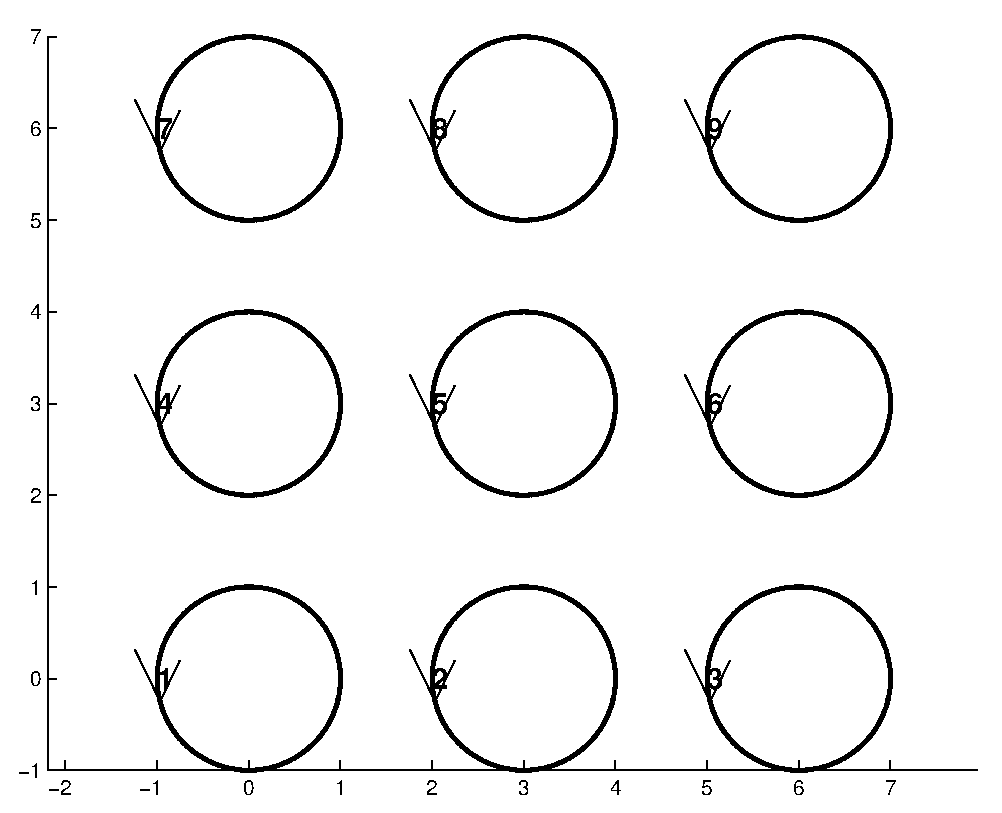
\includegraphics[width=6cm]{circarray}
\caption{An array of $9$ scatterers.}
\label{fig:circarray}
\end{figure}

Let $\Omega$ be the union of disks $D_j$ with radius $r$ whose
midpoints have the coordinates $(an_1^{(j)},an_2^{(j)})\in\mathbb{R}^2$, where
$n_1^{(j)},n_2^{(j)}\in\mathbb{N}$ and $a>0$ is the distance between
two neighboring midpoints. An example for $9$ scatterers is shown in Figure
\ref{fig:circarray}. The PDE is the following.
 
\begin{eqnarray}
\Delta u+k^2u & = & 0  \quad \text{in
}\mathbb{R}^2\backslash\Omega\label{eq:helm0}\\
u&=&0 \quad \text{on } \pO \label{eq:soundsoft0}\\
\frac{\partial u_s}{\partial r}-iku_s & = & o(r^{-1/2}),\label{eq:sommerfeld0}
\end{eqnarray}
Here, $u=u_{inc}+u_s$ is the total field, $u_{inc}$ is the incident
wave, $u_s$ is the scattered field, and $r$ is the radial coordinate.
The Sommerfeld radiation condition
\eqref{eq:sommerfeld} is to be understood to hold uniformly in all
directions. 


We solve the problem using fundamental solutions approximations in
each disk, where the charge  points lie on circles with radius $r_{mfs}<r$.

\subsubsection{Implementation in \mpspack}

\paragraph{Initialization of the problem parameters}

We have the following problem parameters.
\begin{verbatim}
N1=3; N2=3; % Number of scatterers in each direction
r=1; % Radii of circles
a=3; % Distance of midpoints of neighboring circles in each dimension
k=10; % Wavenumber
M=300; % Number of points on each circle
N=150;  % Number of MFS basis fct. in each circle
Rmfs=0.8*r; % Radius of fundamental solutions inside circles
\end{verbatim}

\paragraph{Setup of the geometry}

The geometry is setup using a simple for loop.
\begin{verbatim}
y0=0;
s=segment.empty(N1*N2,0);
for i=1:N1,
    x0=0;
    for j=1:N2
        seg=segment(M,[x0+1i*y0 r 0 2*pi],'p');
        seg.setbc(1,'D',[]);
        s((i-1)*N2+j)=seg;
        x0=x0+a;
    end
    y0=y0+a;
end
\end{verbatim}
In the inner for loop circular segments are created whose handle is
the variable {\texttt seg}. We directly assign the homogeneous
Dirichlet boundary conditions using the command \co{seg.setbc(1,'D',[]);}
The segments are then stored in the array
{\texttt s}. Storing the circular segments in an array makes plotting
easy. Figure \ref{fig:circarray} is simply created with the commands
\begin{verbatim}
o.normals=0;
plot(s,1,o);
\end{verbatim}
Once all segments are created we define the domain by
\co{d=domain([],[],num2cell(s),num2cell(-1*ones(N1*N2,1)));}
This command might look complicated at first because of the use of
{\texttt num2cell}. We need to convert the array {\texttt s} into a
cell structure so that the {\texttt domain} constructor recognizes
that each element of $s$ is a closed shape in itself. Otherwise, the
constructor would try to combine the elements of {\texttt s} into one
connected shape, which is not possible.


\paragraph{Basis functions}

We want to use a basis of fundamental solutions in each of the
circular scatterers. This is achieved with the following for loop.
\begin{verbatim}
x0=0; y0=0; opts.fast=1;
for i=1:N1,
    x0=0;
    for j=1:N2
        Z=@(w) Rmfs*exp(2i*pi*w)+x0+1i*y0;
        Zp=@(w) Rmfs*2i*pi*exp(2i*pi*w);
        d.addmfsbasis({Z,Zp},N,opts);
        x0=x0+a;
    end
    y0=y0+a;
end
\end{verbatim}
The function handle {\texttt Z} defines the fundamental solutions
curve and {\texttt Zp} its derivative. We have to shift the curves
according to the midpoints of the circles.

\paragraph{Solving the problem}
We now have everything together to setup a problem instance.
This is easily done with the {\texttt
  scattering} class and the following three commands.

\begin{verbatim}
pr=scattering(d,[]);
pr.setoverallwavenumber(k);
pr.setincidentwave(-pi/3);
\end{verbatim}

The solution and timing results are then obtained by
\begin{verbatim}
tic; pr.solvecoeffs; fprintf('\tcoeffs done in %.2g sec\n', toc)
fprintf('\tL2 bdry error norm = %g, coeff norm = %g\n', ...
        pr.bcresidualnorm, norm(pr.co));
\end{verbatim}
On a standard Core 2 Duo Laptop this takes just under $40$
seconds with a boundary error of about $2\cdot 10^{-13}$.
We can plot the solution using the following commands.
\begin{verbatim}
o.bb=[-a N2*a -a N1*a];
o.dx=0.05;
o.sepfigs=1;
pr.showthreefields(o);
\end{verbatim}
The command {\tt pr.showthreefields(o)} plots the incoming wave,
scattered field and full field using the parameters given in {\tt
  o}. We have specified {\tt o.sepfigs=1}. This creates three
separate figures for the three different fields instead of plotting
everything into one figure.

\begin{figure}
\center
\begin{tabular}{cc}
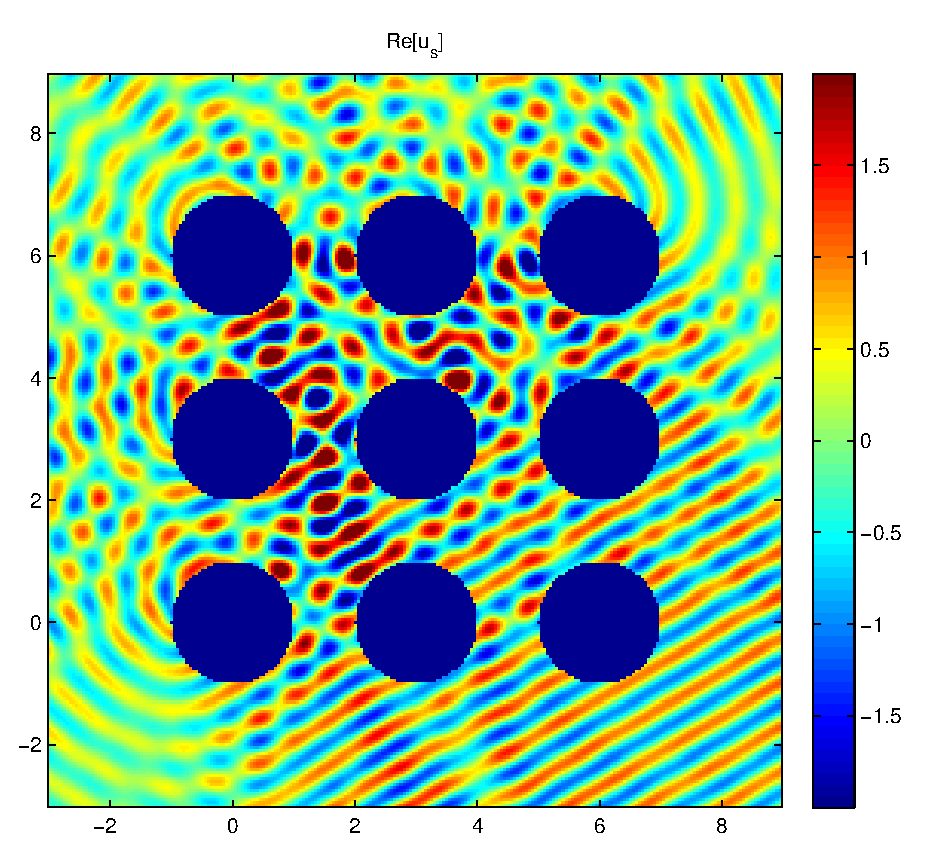
\includegraphics[width=6cm]{circarrayscattered} &
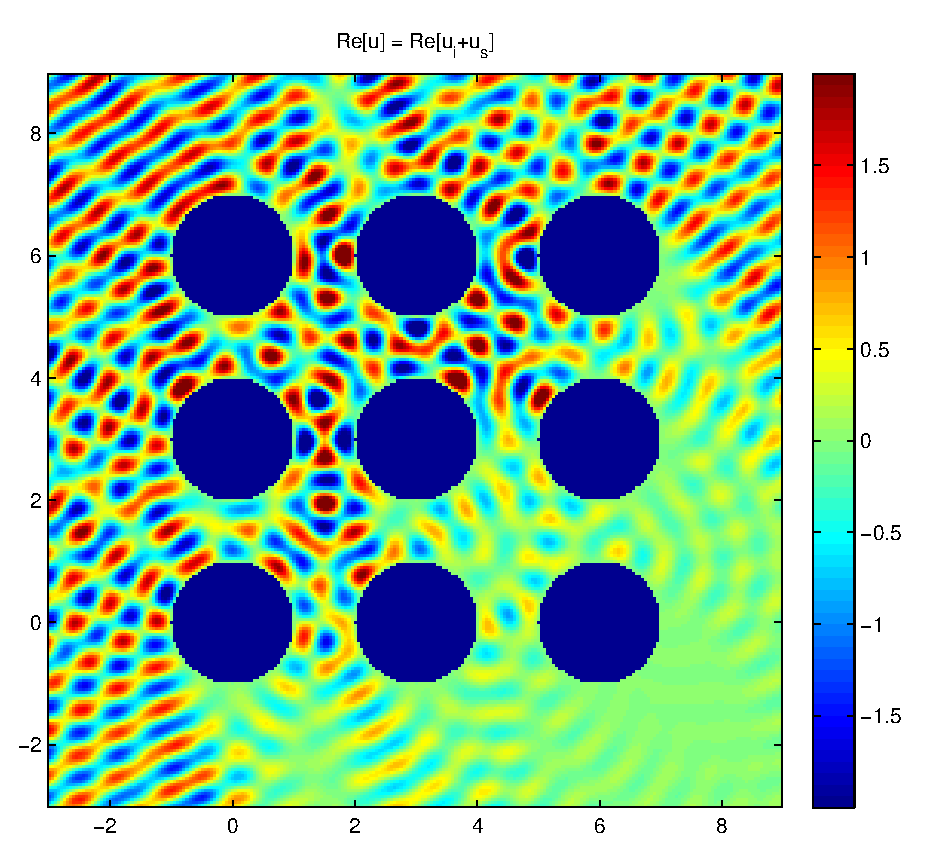
\includegraphics[width=6cm]{circarrayfull}
\end{tabular}
\caption{The scattered (left) and the full field (right) for the
  problem of scattering from an array of circles.}
\label{fig:circarraysol}
\end{figure}


The scattered and the full field are shown in Figure
\ref{fig:circarraysol}. Note that plotting can take a long time since
the array of scatterers spans many wavelenghts for which we need a
sufficiently high resolution. The solution is not symmetric with
respect to the diagonal since the incident angle for the incoming wave is
$-\frac{\pi}{3}$, destroying the symmetry given by the configuration
of scatterers.














\bfi % ffffffffffffffffffffffffffffffffffffffffffffffffffffffffffffffffffffff
\ig{width=\textwidth}{dielhole.eps}
\ca{Transmission scattering (TE-polarized) from dielectric with two inclusions: an air hole
(to the right side) and a `metallic' PMC inclusion (to the left side).
Multiple MFS basis curves are used.
Left: incident wave $u_{inc}$. Center: scattered wave
$u_s$. Right: their sum, the total solution field $u$.}{f:dielhole}
\efi
\bfi % ffffffffffffffffffffffffffffffffffffffffffffffffffffffffffffffffffffff
\bc\ig{width=0.6\textwidth}{dielholegeom.eps}\ec
\ca{MFS curves (red) and boundary curves (blue) used for transmission scattering from dielectric with two inclusions.}{f:dielholegeom}
\efi

% ===========================================================================
\subsection{Transmission scattering with `metal' and air holes}
\label{s:dielhole}

Here we demonstrate how the fundamental solutions introduced in
Sec.~\ref{s:ext} can be used to solve efficiently
the scattering of TE (transverse-electric) polarized $z$-invariant
plane-wave (2D Maxwell equations) from a smooth dielectric body with various
inclusions. We will be somewhat brief in this example.

The mathematical set up is identical to the previous example, except that
there is a bounded dielectric region which has refractive index $n = 1.5$ and
hence a Helmholtz solution with
larger wavenumber than in the surrounding vacuum (or `air').
The field $u$ represents $H_z$, the out-of-plane magnetic field.
The solution in the dielectric must match that in the air at their common
boundary, as we describe shortly. We also have a homogeneous boundary condition
on a `metallic' inclusion inside the dielectric; see Fig.~\ref{f:dielhole}.

First we set up some curves, formed by scaling, translating and rotating
standard `radius-1' segments {\tt 's'} and {\tt 'c'}, and build the
three domains from them,
\begin{verbatim}
s = segment.smoothstar(200, 0.2, 3);          % weak trefoil shape
c = segment.smoothstar(70, 0.1, 2);           % squashed circle

sd = s.scale(2);                              % outer bdry of dielectric
sa = translate(rotate(sm,.3), .8);            % air inclusion bdry
sm = c.scale(0.5); sm.rotate(pi/5); sm.translate(-.8-.6i); % 'metal' bdry

de = domain([], [], sd, -1);                  % exterior air domain
da = domain(sa, 1);                           % air inclusion domain
d = domain(sd, 1, {sm sa}, {-1 -1});          % dielectric w/ 2 holes
d.setrefractiveindex(1.5);                    % choose dielectric index
\end{verbatim}

Assuming relative permeability of unity, the relative
permittivity of the dielectric is $\epsilon = n^2$.
The TE boundary condition is that $u$ is continuous
across a dielectric interface (segments {\tt sd} and {\tt sa}),
while for the normal derivatives $\epsilon^{-1} \partial u/\partial n$ is
continuous.\footnote{See \cite{jackson}.
See {\tt segment.dielectriccoeffs} for where this
is set up in \mpspack.}
We set this up, and a Dirichlet BC on the other inclusion, with,
\begin{verbatim}
setmatch([sd sa], 'diel', 'TE');        % impose TE matching diel-air
sm.setbc(1, 'D', []);                   % Dirichlet (PMC) BC on 'metal'
\end{verbatim}

The domains are then collected into a scattering problem as follows (note
that by including {\tt da} in the first argument list, it is set up as an
`air' domain thus receives a nonzero $u_{inc}$ plane-wave field, although
results are similar if {\tt de} is the only air domain),
\begin{verbatim}
pr = scattering([de da], d);   % includes air pocket in nonzero u_inc
pr.setoverallwavenumber(8);    % incident (air) wavenumber
pr.setincidentwave(-pi/3);     % if just angle given, assumed plane wave
\end{verbatim}

MFS bases are very convenient for such analytic boundaries, and we use the
analytic continuation of the boundary parametrization to generate MFS curves
either inside or outside the actual segment curves
({\tt tau>0} is inside, and {\tt tau<0} outside, for CCW segments).
Fig.~\ref{f:dielholegeom} shows the five MFS curves and the three segments.
The reason the dielectric needs three MFS curves is that (analogous
with Runge's Theorem in complex approximation), singularities are needed in
{\em each} disconnected component of the domain's complement.
The distances {\tt tau} in the following should be chosen as large as possible
while still keeping the coefficient norm {\tt norm(pr.co)} not too large
(i.e.\ $10^4$ or less).
\begin{verbatim}
de.addmfsbasis(sd, 120,struct('tau',0.05));  % exterior domain
da.addmfsbasis(sa, 60, struct('tau',-0.1));  % inside air pocket
d.addmfsbasis(sd,  150,struct('tau',-0.05)); % 1st of 3 curves for diel...
d.addmfsbasis(sm,  60, struct('tau',0.1));   % ...2nd curve in `metal' hole
d.addmfsbasis(sa,  60, struct('tau',0.1));   % ...3rd curve in air hole
\end{verbatim}
Note that the basis set degrees were optimized roughly for this $k$ value,
giving only 450 total degrees of freedom for a problem around
8 wavelengths in size.
Solving for the coefficients of the solution takes 0.67 sec,
\begin{verbatim}
pr.solvecoeffs; pr.bcresidualnorm
\end{verbatim}
The $L^2$ boundary error is less than $10^{-7}$.
We then plot the incident, scattered, and total field as usual with
{\tt pr.showthreefields;} giving Fig.~\ref{f:dielhole}.
Evaluating the solution on a 400$\times$400 grid takes 11 sec.

\subsubsection{Convergence study}
Once a good set of MFS basis sizes has been chosen, as above, they
may all be changed at once conveniently with the {\tt nmultiplier} option.
We could have redone the basis sets as follows,
\begin{verbatim}
d.clearbases; de.clearbases; da.clearbases;
de.addmfsbasis(sd, [], struct('tau',0.05, 'nmultiplier', 120/450));
da.addmfsbasis(sa, [], struct('tau',-0.1, 'nmultiplier', 60/450));
d.addmfsbasis(sd, [],  struct('tau',-0.05,'nmultiplier', 150/450));
d.addmfsbasis(sm, [],  struct('tau',0.1,  'nmultiplier', 60/450));
d.addmfsbasis(sa, [],  struct('tau',0.1,  'nmultiplier', 60/450));
\end{verbatim}
The mutipliers were set up to be the fraction of the total degrees of freedom
that they were before, but now they can be scaled with a single command,
viz, {\tt pr.updateN(450)} sets up the original basis sizes,
as may be checked with {\tt diff([pr.basnoff pr.N])} which gives the
numbers of degrees of freedom in each problem basis set.
We put this in a convergence loop,
\begin{verbatim}
Ns=300:50:600; for i=1:numel(Ns)
  pr.updateN(Ns(i)); pr.solvecoeffs; u0 = pr.pointsolution(pointset(0));
  fprintf('N=%d, co-norm=%g, bc-norm=%g, |u(0)|=%.16g\n', Ns(i), ...
          norm(pr.co), pr.bcresidualnorm, abs(u0));
end
\end{verbatim}
We actually doubled the number of quadrature points on the original
segments to perform this high-accuracy study, giving 680 quadrature points in
total.
The output shows very rapid convergence,
\begin{verbatim}
N=300, co-norm=2125.38, bc-norm=0.000363003, |u(0)|=3.045222448551815
N=350, co-norm=1968.37, bc-norm=1.26165e-05, |u(0)|=3.045222451567895
N=400, co-norm=1844.05, bc-norm=4.21908e-07, |u(0)|=3.045222451435764
N=450, co-norm=1746.25, bc-norm=9.77848e-08, |u(0)|=3.045222451435782
N=500, co-norm=1651.79, bc-norm=3.96167e-09, |u(0)|=3.045222451436035
N=550, co-norm=1581.87, bc-norm=1.1487e-09,  |u(0)|=3.045222451436006
N=600, co-norm=1521.16, bc-norm=1.44025e-10, |u(0)|=3.045222451436037
\end{verbatim}
This suggests that, at least for $u$ at the origin, we had 12 correct
digits in the solution with the total $N=450$ used above,
and probably achieved 14 digits with $N=600$,
computed in just a couple of seconds.




% ===========================================================================
\subsection{Acoustic scattering from the unit square}
\label{s:square}

This example introduces a new feature: the use of decomposition
of a region of constant wavenumber into computational subdomains connected
by fictitious boundaries. The code is in \verb?examples/tut_square.m?

\subsubsection{Problem description and solution approach}
\label{s:scatbvp}

In this example we solve the problem of time-harmonic 
acoustic sound-soft scattering from the unit square $\Omega=(-0.5,0.5)^2$.
The full PDE has the following form.
\begin{eqnarray}
\Delta u+k^2u & = & 0  \quad \text{in
}\mathbb{R}^2\backslash\Omega\label{eq:helm}\\
u&=&0 \quad \text{on } \pO \label{eq:soundsoft}\\
\frac{\partial u_s}{\partial r}-iku_s & = & o(r^{-1/2}),\label{eq:sommerfeld}
\end{eqnarray}
Here, $u=u_{inc}+u_s$ is the total field, $u_{inc}$ is the incident
wave, $u_s$ is the scattered field, and $r$ is the radial coordinate.
The Sommerfeld radiation condition
\eqref{eq:sommerfeld} is to be understood to hold uniformly in all
directions. 

\begin{figure}
\center
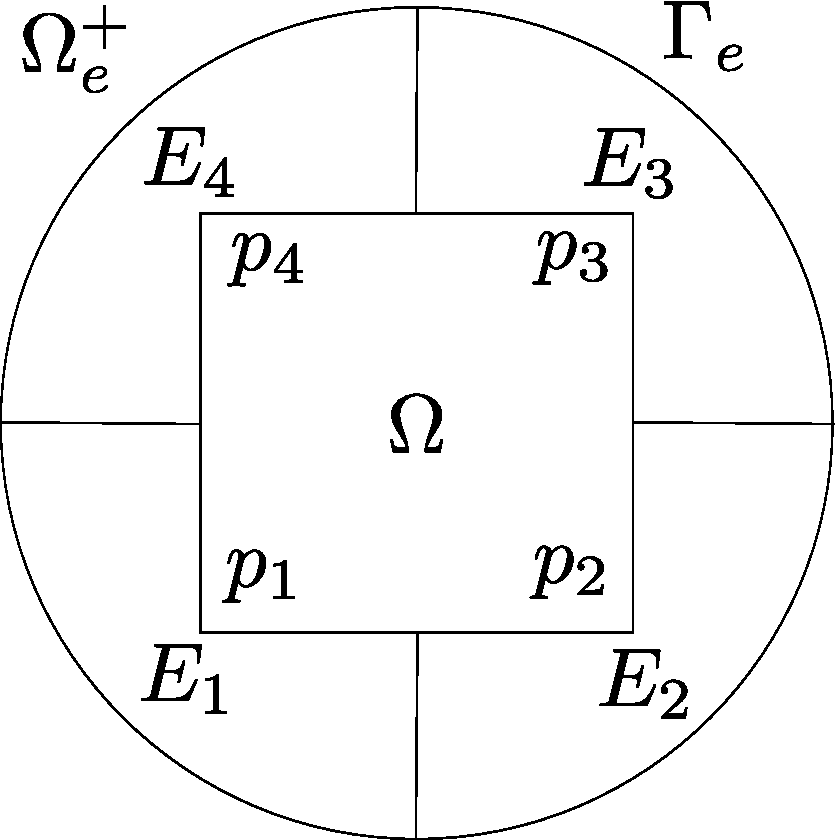
\includegraphics[width=6cm]{geometry}
\vspace{-.5cm}
\caption{Geometry of the problem}
\label{fig:geom}
\end{figure}


To achieve high accuracy we cannot simply use fundamental solutions
to approximate the scattered field. The problem is the singularities
of the solution $u$ at the corners. If these are not represented in
the basis our approximation error will decay very slowly as the number
of basis functions increases. To solve this problem we use the domain
decompositon shown in Figure \ref{fig:geom}. The idea is that each of
the elements $E_i$ only contains one corner $p_i$ of the square. We can then
match the corner behavior in each domain by using fractional order
Bessel functions. Since furthermore, $u=0$ on $\partial\Omega$ it will
be sufficient to use Fourier-Bessel sine functions that automatically
satisfy the zero boundary conditions on the sides of the square.
Hence, the total field $u$ is approximated in each element $E_i$ using
an approximation of the form
$$
u(r,\theta)\approx
\sum_{j=1}^{N_i}c_j^{(i)}J_{\frac{2}{3}j}(kr)\sin(\frac{2j}{3}\theta).
$$
The polar coordinate system in each element $E_i$ is rotated in such a way
that the basis functions are zero on the sides adjacent to the corner
at $p_i$.

In the infinite domain $\Omega_e^+$ we use a basis of fundamental
solutions to represent the scattered field $u_s$. Hence, for
$\bx\in\Omega^+$ we have
$$
u_s(\bx)\approx \sum_{j=1}^{N_e}\frac{i}{4}c_j^{(e)}H_0^{(1)}(|\bx-\by_j|),
$$
where $\by_j=r_{mfs}e^{i\phi_j}$ and $\phi_j=\frac{2\pi j}{N_e}$. Note
that we approximate with the fundamental solutions the scattered field
$u_s$ while in the finite subdomains $E_i$ we approximate the total
field $u$. The compatibility conditions between approximations $u^{i}$
und $u^{j}$ in two neighboring elements $E_i$ and $E_j$ with common
boundary $\Gamma_{ij}$ are given by
$$
u^{(i)}(\bx)\approx u^{(j)}(\bx),\quad \frac{\partial u}{\partial
  n_i}{u^{(i)}}(\bx)\approx  \frac{\partial u}{\partial
  n_i}{u^{(j)}}(\bx),
$$
where $\bx\in\Gamma_{ij}$ and $\frac{\partial}{\partial\nu_i}$ is the
outward normal derivative at the boundary of $E_i$.
On the interface $\Gamma_{ie}$ between an element $E_i$ and the
exterior domain $\Omega_e^{+}$ we have the compatibility conditions
$$
u^{(i)}(\bx)\approx u_{inc}(\bx)+u_s^{(e)}(\bx),\quad \frac{\partial}{\partial
  n_i}{u^{(i)}}(\bx)\approx  \frac{\partial}{\partial
  n_i}{(u_s^{(e)}+u_{inc})}(\bx),
$$
where $u_s^{(i)}$ is the fundamental solutions approximation to the
scattered field in $\Omega_e^{+}$. We have to add the incident field
to the approximate scattered field since we are matching with the
total field in the elements $E_i$.
An approximate solution to the whole problem is now 
computed by minimizing the $L^2$ error of 
the compatibility conditions on all interfaces.

\subsubsection{Implementation in \mpspack}

Although the setup of the problem seems quite complicated we will see
that it is very simple to set it up in \mpspack. Indeed, the most part
of the code will be devoted to creating the mesh structure from
Figure \ref{fig:geom}.

\paragraph{Initialization of the problem parameters}

We need to define the following problem parameters.
\begin{verbatim}
k = 50;      % Wavenumber
r = 1.0;     % Radius of outer circle    
M = 200;     % Number of quadrature points on segments
N=100;       % Number of basis fct. in each subdomain
a=.5;        % Half-Size of the square
rmfs=0.8*r;  % Radius of the fundamental solutions curve
\end{verbatim}


\paragraph{Setup of the geometry}

We now need to define the geometry. Fortunately,
\mpspack\ gives some support for the construction of the geometry.

The list of segments is defined by the following three commands.

\begin{verbatim}
s = segment.polyseglist(M, [1i*r 1i*a a+1i*a a r]);
s=[s(1:3) segment(2*M, [0 r 0 pi/2])];
s = [s rotate(s, pi/2) rotate(s, pi) rotate(s, 3*pi/2)];
\end{verbatim}
The first command defines all the straight lines that form part of the
boundary of $E_3$. For this we use {\texttt{polyseglist}}. The command
{\texttt polyseglist} constructs a closed polygon. We then delete the
last two segments of the array {\texttt s} and add instead the
circular line segment. This results in the segments shown in the left
plot of Figure \ref{fig:circelem}. We now rotate this element three times to
obtain the segments showin in the right plot of Figure \ref{fig:circelem}.
\begin{figure}
\begin{tabular}{cc}
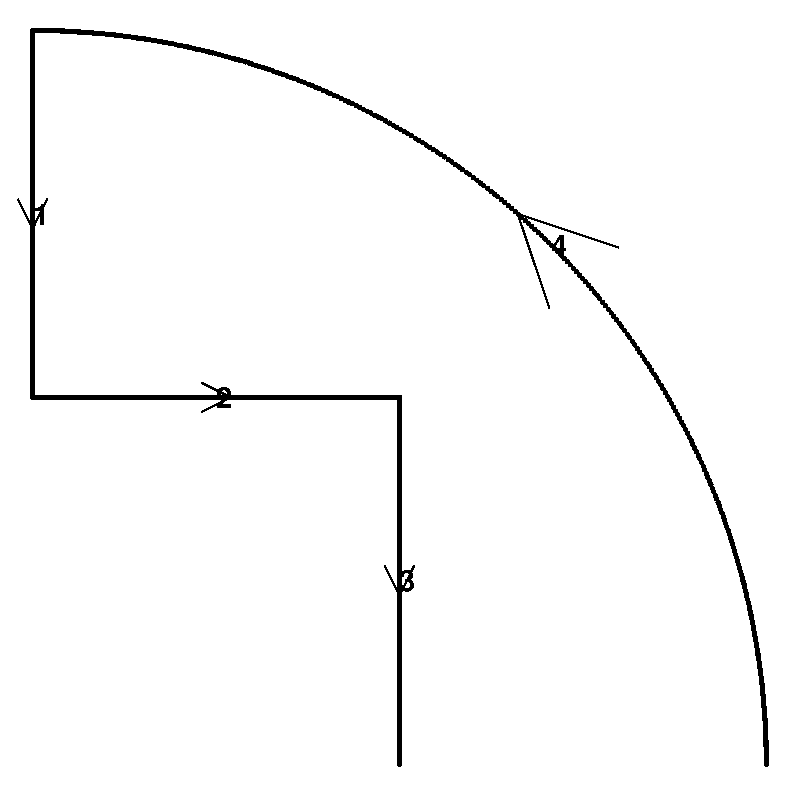
\includegraphics[width=5cm]{circelem1} &
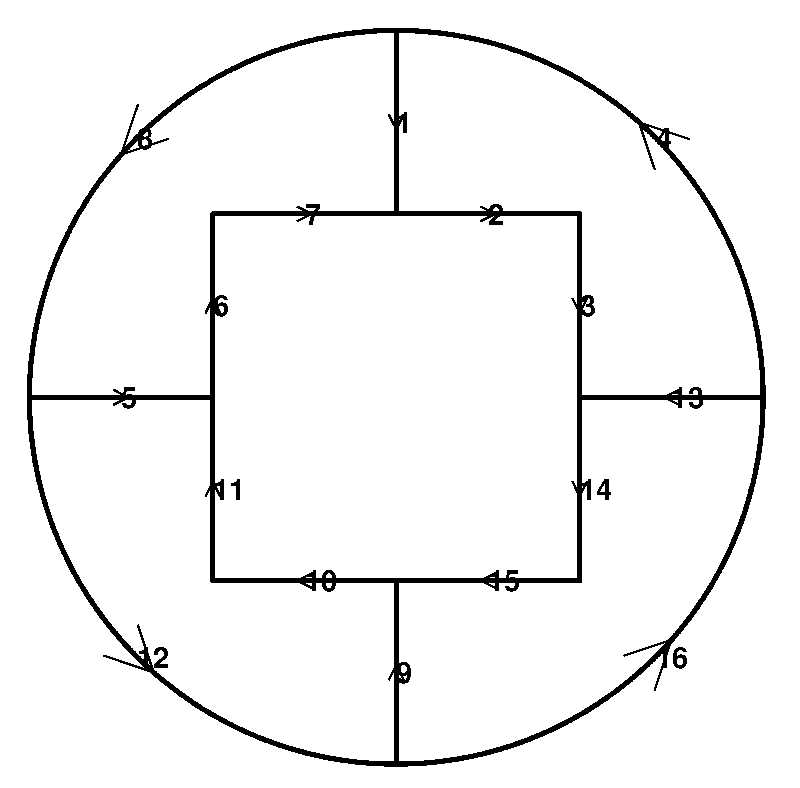
\includegraphics[width=5cm]{circelem2}
\end{tabular}
\caption{The segments in the right plot are created by rotating the segments
  shown in the left plot.}
\label{fig:circelem}
\end{figure}

For later it is important to have a separate list of all segments not
belonging to the square and all segments belonging to the outer
circle.

\begin{verbatim}
sdecomp=s([1 4 5 8 9 12 13 16]); % All artificial boundaries
extlist=s([4 8 12 16]);          % Segments forming the outer circle
\end{verbatim}

We now define the domains. By taking the rotational symmetry into
account we can do this in a simple for loop.

\begin{verbatim}
d=domain.empty(4,0);
for j=1:4, d(j)=domain(s(1+mod(4*(j-1)+[0 1 2 12 3],16)),[1 1 1 -1 1]); end
ext = domain([], [],extlist(end:-1:1), -1); 
\end{verbatim}
The for loop looks slightly complicated. But all it does is pick out
the right indices for the elements forming a domain and creating it
together with the right sense of direction. At the end we have an
array {\texttt d} containing the four fine domains $E_i$. The exterior
domain {\texttt ext} is created by traversing {\texttt extlist} in
reverse order with reversed sense $-1$. This is necessary since we now
have the boundary of an exterior domain, which has a reversed sense of
direction.

\paragraph{Boundary conditions and basis functions}

Setting up the compatibility conditions between the elements is 
trivial. It is done by
the command
\begin{verbatim}
sdecomp.setmatch([k -k],[1 -1]);
\end{verbatim}
The matching conditions for the function values are scaled by the
wavenumber $k$ to balance the different scaling between the $L^2$ error
in the function and the $L^2$ error in the
derivative.\footnote{Consider the one dimensional plane wave
  $e^{ikx}$. The derivative is $ike^{ikx}$. Hence, in general it makes sense to
  scale the $L^2$ error of function values by $k$ to give it the same
  dimension as the $L^2$ error of the derivative.}

We can now add the basis functions to the domains. The fractional
Bessel functions are added to the interior domains by the following
command.
\begin{verbatim}
nuopts=struct('type','s','cornermultipliers',[0 0 1 0 0],'rescale_rad',1);
for j=1:4, d(j).addcornerbases(N,nuopts); end
\end{verbatim}
The options structure {\texttt nuoopts} specifies that we only want
Fourier-Bessel sine functions at the third corner of each domain. This
is the corner belonging to the square. The option {\texttt
  'rescale\_rad'} specifies that the basis functions are rescaled to
balance out the bad scaling of Bessel functions. The method {\texttt
  addcornerbases} automatically finds out the right fractional orders,
offsets and suitable branch vectors.

The exterior fundamental solutions are added with the following command.
\begin{verbatim}
Z=@(t) rmfs*exp(2i*pi*t); Zp=@(t) 2i*pi*rmfs*exp(2i*pi*t);
opts=struct('eta','k','fast',1,'nmultiplier',2);
ext.addmfsbasis({Z, Zp},N,opts);
\end{verbatim}
Note that now {\texttt nmultiplier} is set to $2$. It turns out to be
effective for this problem to use twice as many fundamental solutions
as there are Fourier-Bessel sine functions in each domain.

\paragraph{Solving the problem}
We now have everything together to setup the problem class and solve
the scattering problem. The following commands setup the scattering
problem and define an incident plane wave.
\begin{verbatim}
pr=scattering(ext,d);
pr.setoverallwavenumber(k);
pr.setincidentwave(-pi/4);
\end{verbatim}
There is one small specialty here. In the first line we have 
defined {\texttt ext} to be an air-domain and the array {\texttt d} to
be a non-air domain. This tells \mpspack\ to add the incident field to
the exterior basis functions in assembling the least-squares
problem. In the finite domains this is not necessary since there we
approximate directly the full field.



The following commands now solve the problem and plot the solution
$u$.
\begin{verbatim}
tic; pr.solvecoeffs; fprintf('\tcoeffs done in %.2g sec\n', toc)
fprintf('\tL2 bdry error norm = %g, coeff norm = %g\n', ...
        pr.bcresidualnorm, norm(pr.co))
o.bb=[-1.5 1.5 -1.5 1.5];
o.dx=0.02;

[ui gx gy] = pr.gridincidentwave(o);
u = pr.gridsolution(o);

figure;
imagesc(gx, gy, real(ui+u)); title('Full Field (Real Part)');
c = caxis; caxis([-1 1]*max(c));
axis equal tight;
colorbar;
set(gca,'ydir','normal'); 
\end{verbatim}
The incident field {\texttt ui} 
is automatically evaluated only in air-domains. If
we want to evaluate it in all domains we have to set {\texttt
  o.all=1}. But here the default behavior is fine for us. The sum
{\texttt ui+u} is now the total field in all domains (remember that
{\texttt u} approximates the total field in the interior domains
and the scattered field in the exterior domain). The {\texttt
  scattering} class also provides a routine {\texttt showthreefields}
to plot the incident wave, scattered field and total field. However,
the routine assumes that the computed solution is the scattered field,
which is not correct for the way we have set up this problem. The
resolution if the plot can easily be increased by decreasing the
variable {\texttt o.dx}, which influences the distance of two grid points.


The output of the example problem is shown in Figure \ref{fig:squareplot}.
\begin{figure}
\center
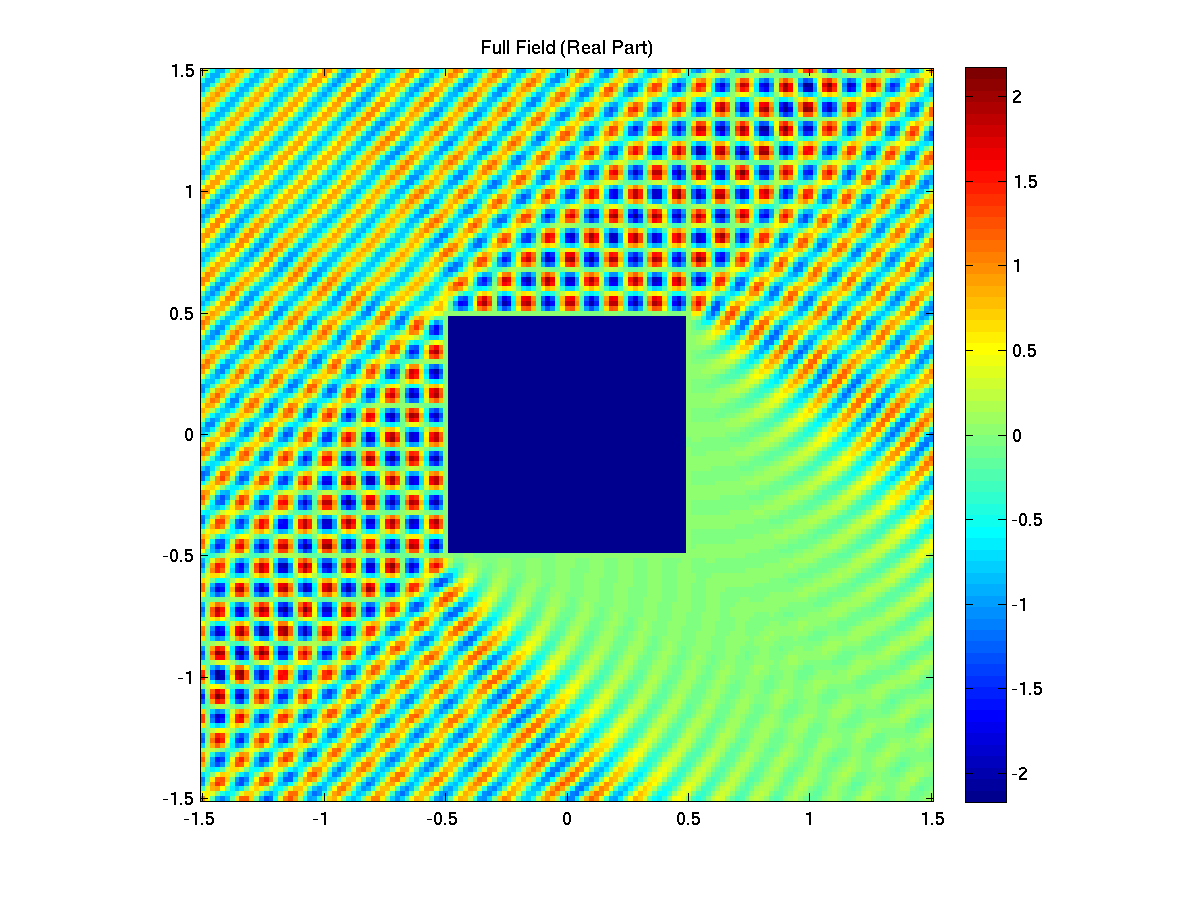
\includegraphics[width=8cm]{squareplot}
\caption{The solution of the scattering problem on the unit
  square with sound-soft boundary conditions.}
\label{fig:squareplot}
\end{figure}
The $L^2$ boundary error of the solution is approximately $1.5\cdot
10^{-10}$. On a standard laptop with Intel Core 2 Duo processor the
solution vector is computed in around $11$ seconds. The plot takes
slightly longer.

A wonderful feature of this approach is that we can trivially switch
to a sound-hard scattering problem, that is instead of requiring $u=0$
on $\partial\Omega$ we require $\frac{\partial}{\partial n} u=0$ on
$\partial\Omega$. All we have to do is switch to Fourier-Bessel cosine
functions. These automatically satisfy the required condition for the
normal derivative. The solution to this problem is shown in Figure
\ref{fig:squareplot2}.
\begin{figure}
\center
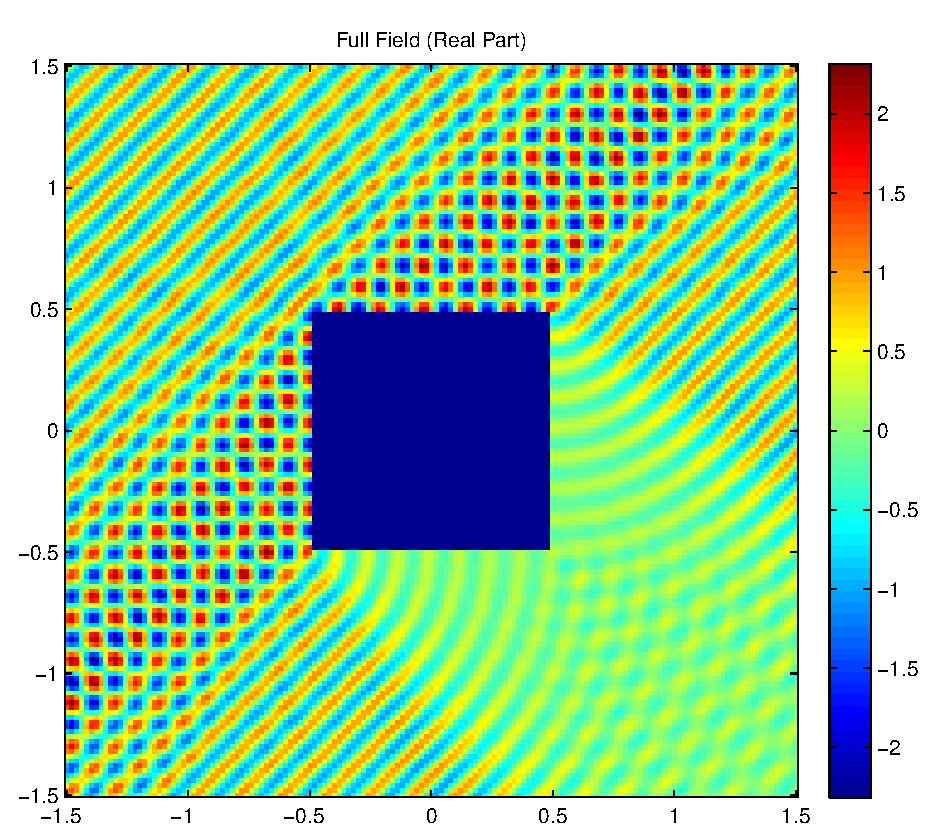
\includegraphics[width=8cm]{squareplot2}
\caption{The solution of the scattering problem on the unit
  square with sound-hard boundary conditions.}
\label{fig:squareplot2}
\end{figure}
The accuracy and solution time are comparable to the sound-soft
scattering case.

%%% Local Variables: 
%%% mode: latex
%%% TeX-master: "tutorial"
%%% End: 

